\section{Qualità visiva dei risultati ottenuti}
\label{sec:chapter_prove_sperimentali_qualita_visiva}

In questo paragrafo vengono mostrate i risultati visivi ottenuti da due differenti scene sottoposte ad ogni fase del servizio implementato in questo lavoro di tesi.
\\ 
Il servizio in particolare ha permesso la creazione della struttura dell’appartamento, l’arredamento, l’applicazione di luci ed ombre tramite lightmap e l’applicazione di effetti di riflessione e rifrazione tramite envmap.
\\
Per la prima scena realizzata è stato utilizzato come riferimento un ambiente domestico a due piani realmente esistente.
\\
La macchina su cui è stato avviato il servizio di Bake presenta le seguenti caratteristiche:
\begin{itemize}
\item Processore: 3,6 GHz Intel Core i7-3820.
\item Scheda grafica: NVIDIA GeForce GTX 670.
\item Memoria RAM: 16 GB.
\end{itemize}
In particolare il servizio di bake  è stato avviato con un valore di sample pari a 300 ed ha impiegato 9 ore e 57 minuti per il calcolo di luci ed ombre realistiche.
\\
Nelle figure vengono mostrati i risultati visivi ottenuti e, quando possibile, vengono mostrati dei confronti diretti tra le foto dell'ambiente domestico reale, utilizzata come riferimento, e la scena virtuale.
\begin{figure}[htb]
 \centering
 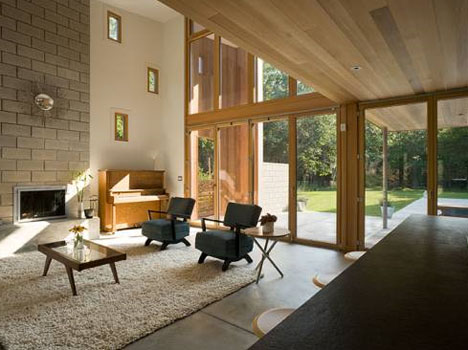
\includegraphics[width=0.9\linewidth]{images/chapter_prove_sperimentali/scena1_reale.jpg}\hfill
 \caption[Ambiente reale: Salone, veduta 1]{Foto reale del salone utilizzata come riferimento (veduta 1).}
 \label{fig:prove_sperimentali_qualita_visiva_scena1_reale}
\end{figure}
\begin{figure}[htb]
 \centering
 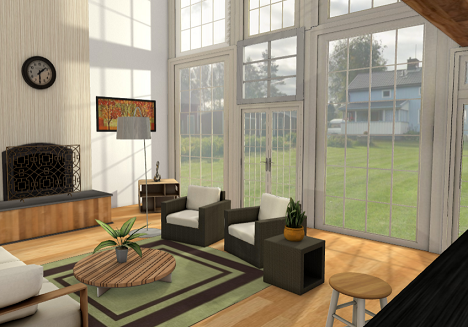
\includegraphics[width=0.9\linewidth]{images/chapter_prove_sperimentali/scena1_bake.png}\hfill
 \caption[Ambiente virtuale: Salone primo piano, veduta 1]{Immagine del salone (primo piano) costruito nell'editor e processato dal servizio di bake (veduta 1).}
 \label{fig:prove_sperimentali_qualita_visiva_scena1_bake}
\end{figure}
\begin{figure}[htb]
 \centering
 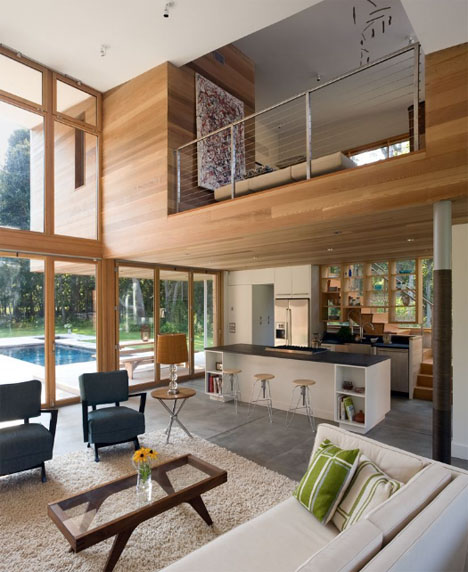
\includegraphics[width=1\linewidth]{images/chapter_prove_sperimentali/scena2_reale.jpg}\hfill
 \caption[Ambiente reale: Salone primo piano, veduta 2]{Foto reale del salone (primo piano) utilizzata come riferimento (veduta 2). L'immagine permette di osservare l'angolo cottura, le scale ed una porzione del piano superiore.}
 \label{fig:prove_sperimentali_qualita_visiva_scena2_reale}
\end{figure}
\begin{figure}[htb]
 \centering
 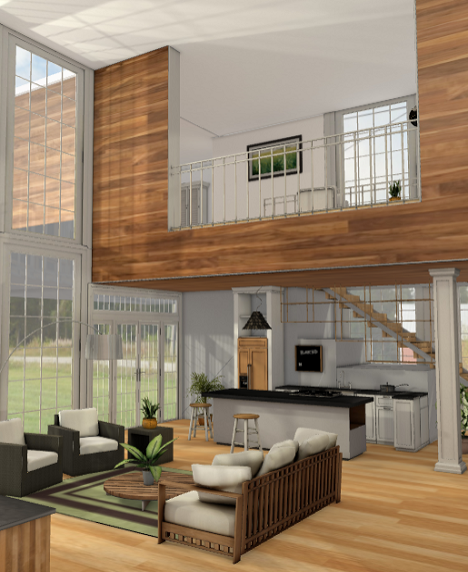
\includegraphics[width=1\linewidth]{images/chapter_prove_sperimentali/scena2_bake.png}\hfill
 \caption[Ambiente virtuale: Salone primo piano, veduta 2]{Immagine del salone (primo piano) costruito nell'editor e processato dal servizio di bake (veduta 2).}
 \label{fig:prove_sperimentali_qualita_visiva_scena2_bake}
\end{figure}
\begin{figure}[htb]
 \centering
 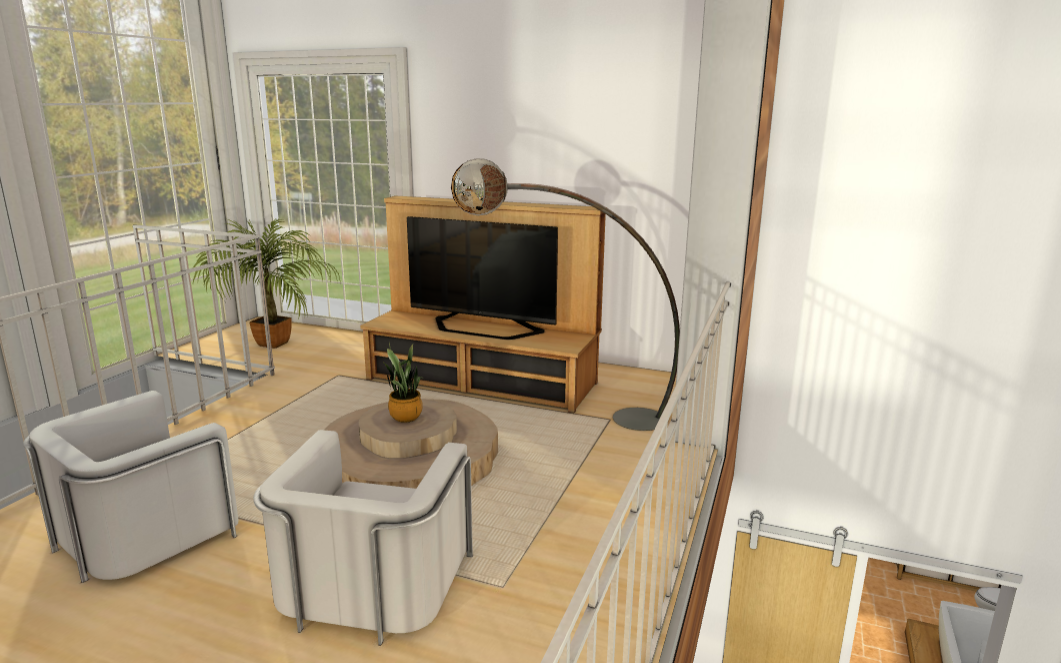
\includegraphics[width=1\linewidth]{images/chapter_prove_sperimentali/scena_1_pianosup_hobby.png}\hfill
 \caption[Ambiente virtuale: Sala relax secondo piano, veduta 1]{Immagine della sala relax (secondo piano) costruita nell'editor e processato dal servizio di bake. La foto mette in risalto le ombre proiettate sul muro.}
 \label{fig:prove_sperimentali_qualita_visiva_scena_hobby1}
\end{figure}
\begin{figure}[htb]
 \centering
 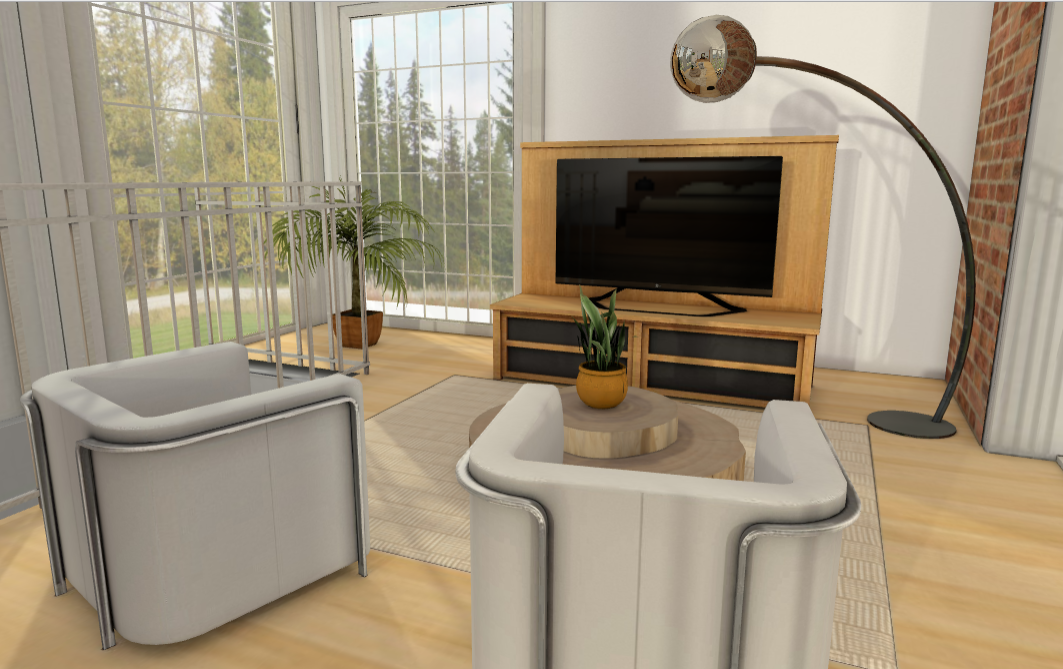
\includegraphics[width=1\linewidth]{images/chapter_prove_sperimentali/scena_2_pianosup_hobby.png}\hfill
 \caption[Ambiente virtuale: Sala relax secondo piano, veduta 2]{Immagine della sala relax (secondo piano) costruita nell'editor e processato dal servizio di bake. La foto mette in risalto i riflessi proiettati dal televisore e dalla lampada.}
 \label{fig:prove_sperimentali_qualita_visiva_scena_hobby2}
\end{figure}
\begin{figure}[htb]
 \centering
 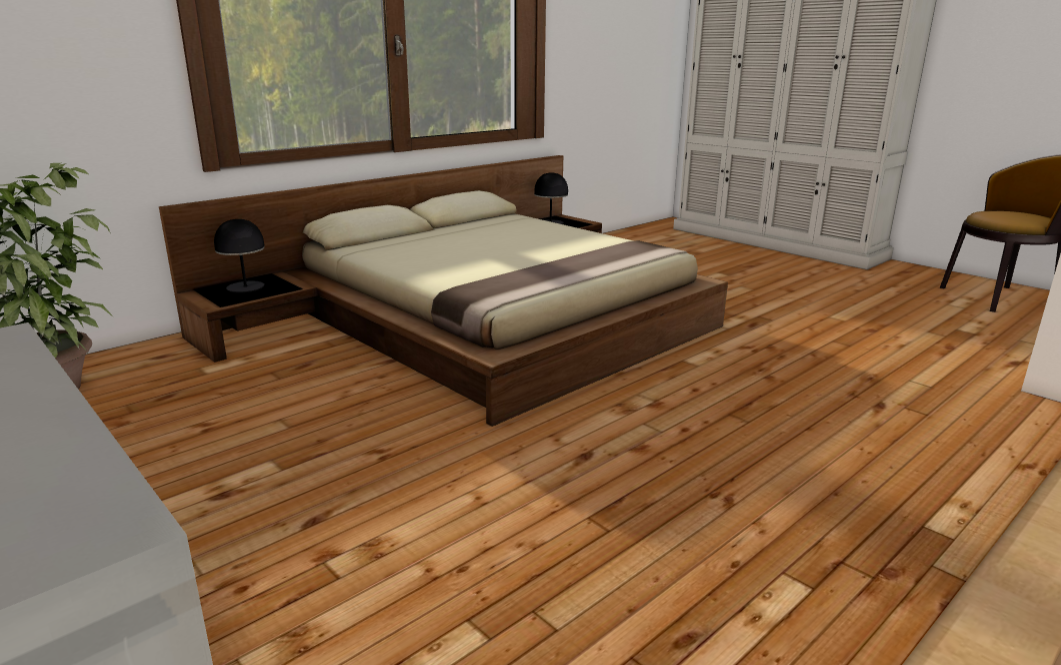
\includegraphics[width=1\linewidth]{images/chapter_prove_sperimentali/scena_1_pianosup_letto.png}\hfill
 \caption[Ambiente virtuale: Camera letto secondo piano]{Immagine della camera da letto (secondo piano) costruita nell'editor e processato dal servizio di bake.}
 \label{fig:prove_sperimentali_qualita_visiva_scena_hobby3}
\end{figure}
\begin{figure}[htb]
 \centering
 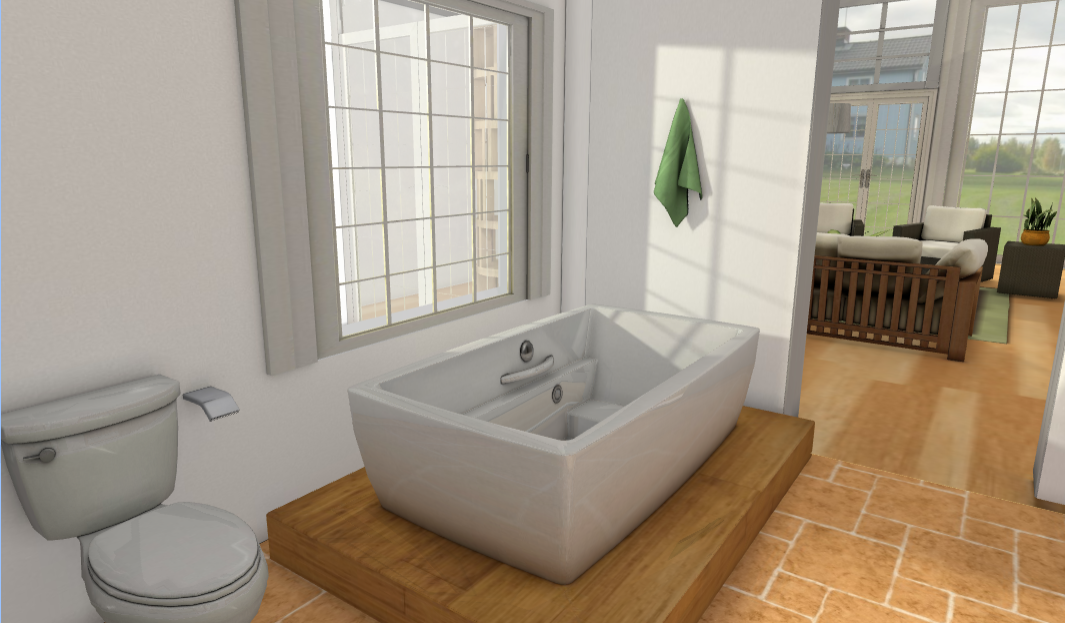
\includegraphics[width=1\linewidth]{images/chapter_prove_sperimentali/scena_bagno.png}\hfill
 \caption[Ambiente virtuale: Bagno primo piano]{Immagine del bagno (primo piano) costruita nell'editor e processato dal servizio di bake.}
 \label{fig:prove_sperimentali_qualita_visiva_scena_hobby4}
\end{figure}
\\
Invece le immagini \ref{fig:prove_sperimentali_qualita_visiva_ufficio_1} \ref{fig:prove_sperimentali_qualita_visiva_ufficio_2} \ref{fig:prove_sperimentali_qualita_visiva_ufficio_3} \ref{fig:prove_sperimentali_qualita_visiva_ufficio_hobby} rappresentano una seconda scena; un open space lavorativo comprensivo di area relax.
Per la realizzazione di questa scena, il servizio di bake  è stato avviato con un valore di sample pari ad 80 ed ha impiegato circa 3 ore per il calcolo di luci ed ombre realistiche.
\\
\begin{figure}[htb]
 \centering
 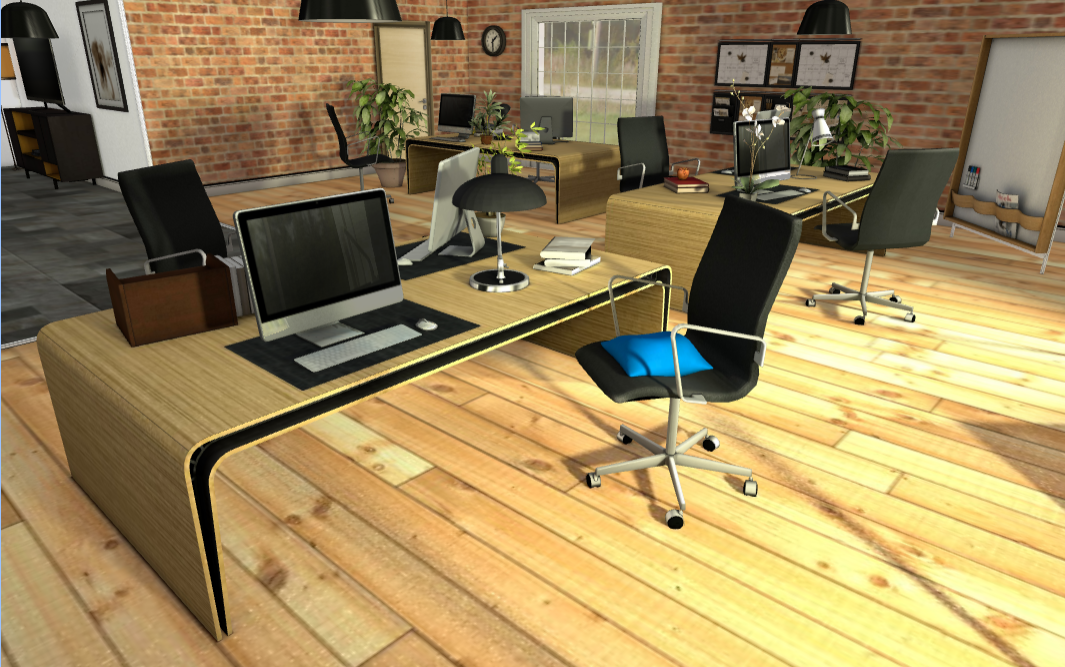
\includegraphics[width=0.9\linewidth]{images/chapter_prove_sperimentali/scena_office_vista1.png}\hfill
 \caption[Ambiente virtuale: Ufficio, veduta 1]{Immagine dell'ufficio costruita nell'editor e processato dal servizio di bake (veduta 1). La foto mette in risalto l'ombra proiettate, in particolare quella sul cuscino blu, ed i riflessioni del computer.}
 \label{fig:prove_sperimentali_qualita_visiva_ufficio_1}
\end{figure}
\begin{figure}[htb]
 \centering
 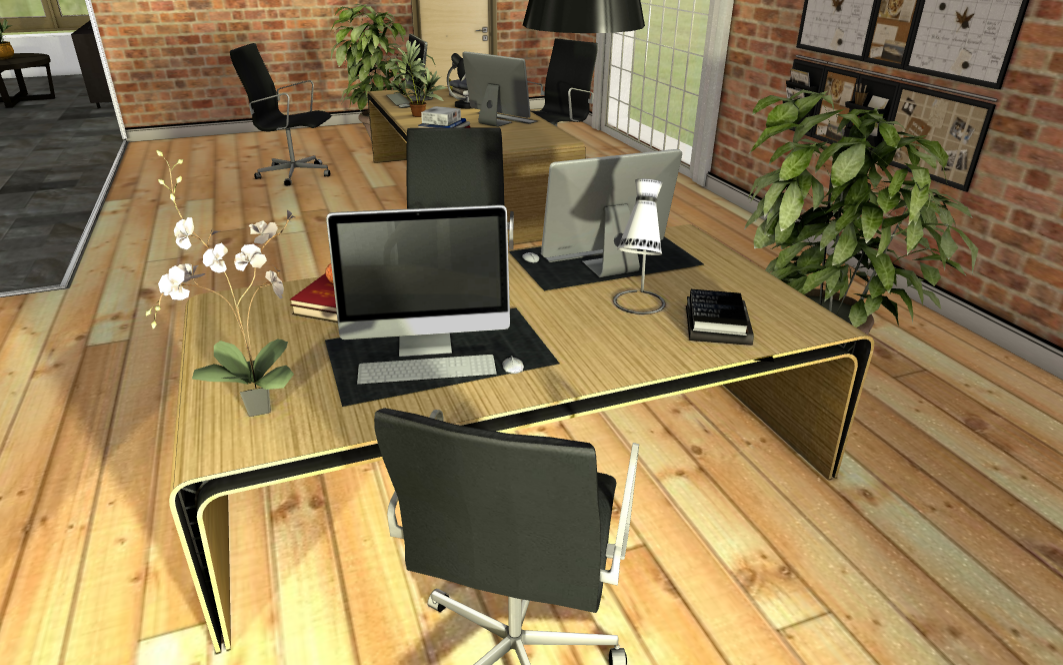
\includegraphics[width=0.9\linewidth]{images/chapter_prove_sperimentali/scena_office_vista2.png}\hfill
 \caption[Ambiente virtuale: Ufficio, veduta 2]{Immagine dell'ufficio costruita nell'editor e processato dal servizio di bake (veduta 2). La foto mette in risalto l'ombra proiettate, in particolare quella dalla lampada, ed i riflessioni proiettati dal computer.}
 \label{fig:prove_sperimentali_qualita_visiva_ufficio_2}
\end{figure}
\begin{figure}[htb]
 \centering
 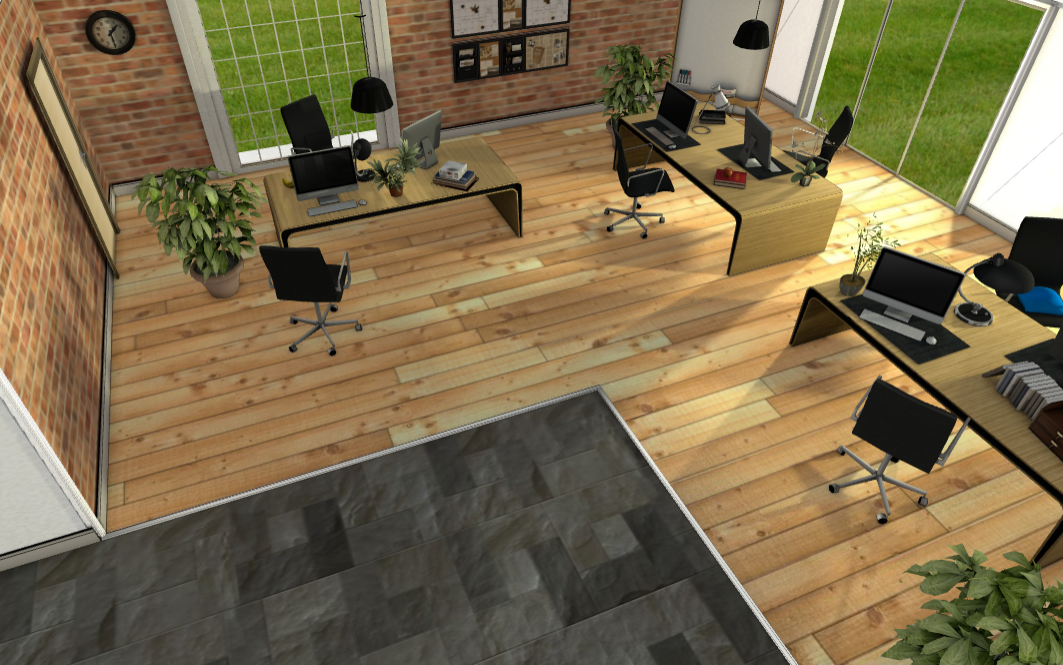
\includegraphics[width=0.9\linewidth]{images/chapter_prove_sperimentali/scena_office_vista4.png}\hfill
 \caption[Ambiente virtuale: Ufficio, veduta 3]{Immagine dell'ufficio costruita nell'editor e processato dal servizio di bake (veduta 3). La foto mette in risalto le principali ombre proiettate dalla sala.}
 \label{fig:prove_sperimentali_qualita_visiva_ufficio_3}
\end{figure}
\begin{figure}[htb]
 \centering
 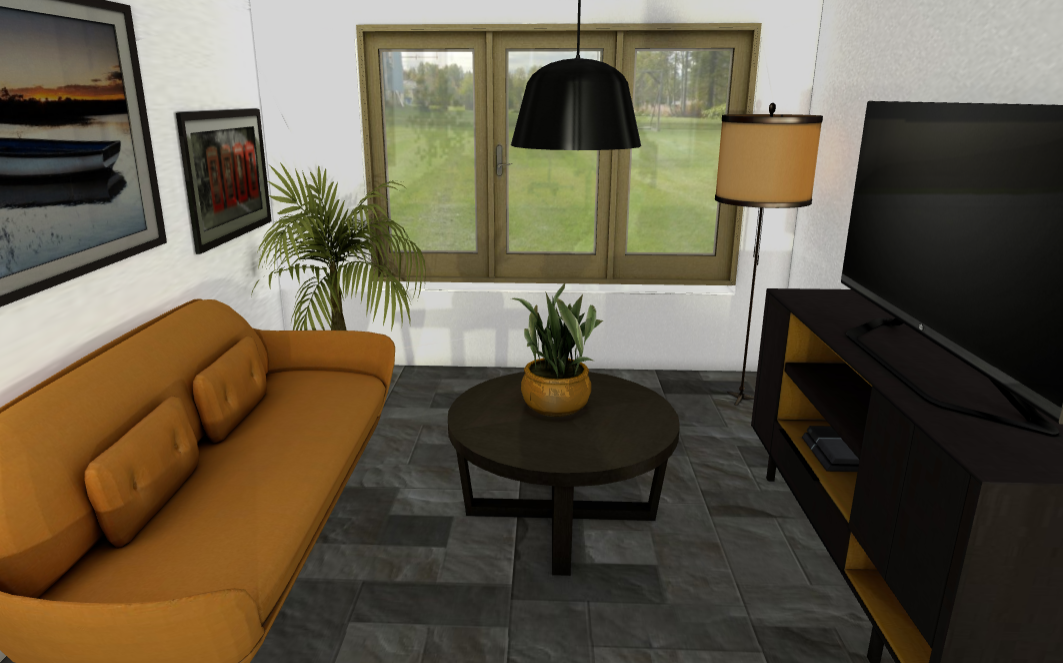
\includegraphics[width=0.9\linewidth]{images/chapter_prove_sperimentali/scena_office_hobby.png}\hfill
 \caption[Ambiente virtuale: Ufficio sala hobby]{Immagine della sala hobby nell'ufficio costruita nell'editor e processato dal servizio di bake. La foto mette in risalto l'ombra proiettate ed i riflessioni proiettati dal televisore, il vaso, il vetro ed i quadri.}
 \label{fig:prove_sperimentali_qualita_visiva_ufficio_hobby}
\end{figure}